\documentclass{article}
\usepackage[utf8]{inputenc}
\usepackage{pgfplots}
\pgfplotsset{width=10cm,compat=1.9}
\usepackage{amsmath,amssymb,amsthm}
\usepackage{graphicx}
\usepackage{float}
\usepackage{blindtext}
\usepackage{hyperref}
\usepackage{verbatim}
\usepackage{gensymb}
\usepackage{enumerate}
\usepackage{graphicx}
\hypersetup{
    colorlinks=true,
    linkcolor=blue,
    filecolor=magenta,      
    urlcolor=cyan,
    pdftitle={Overleaf Example},
    pdfpagemode=FullScreen,
    }
\usepackage[slovene]{babel}

\setlength{\parindent}{0pt}
\setlength{\parskip}{4pt}

\newcounter{example}[section]
\newenvironment{example}[1][]{\refstepcounter{example}\par\medskip
   \noindent \textbf{Naloga~\theexample. #1} \rmfamily}{\medskip}

\newtheorem*{zgled}{Zgled}

\title{Geometrija}
\author{Bor Bregant}
\date{\vspace{-5ex}}

\begin{document}

\maketitle

\section{Štirikotnik in pravilni $n$-kotnik}

Vsota notranjih kotov štirikotnika je $360\degree$. \textit{dokaz s triangulacijo}

\subsection*{Paralelogram}

\begin{figure}[H]
    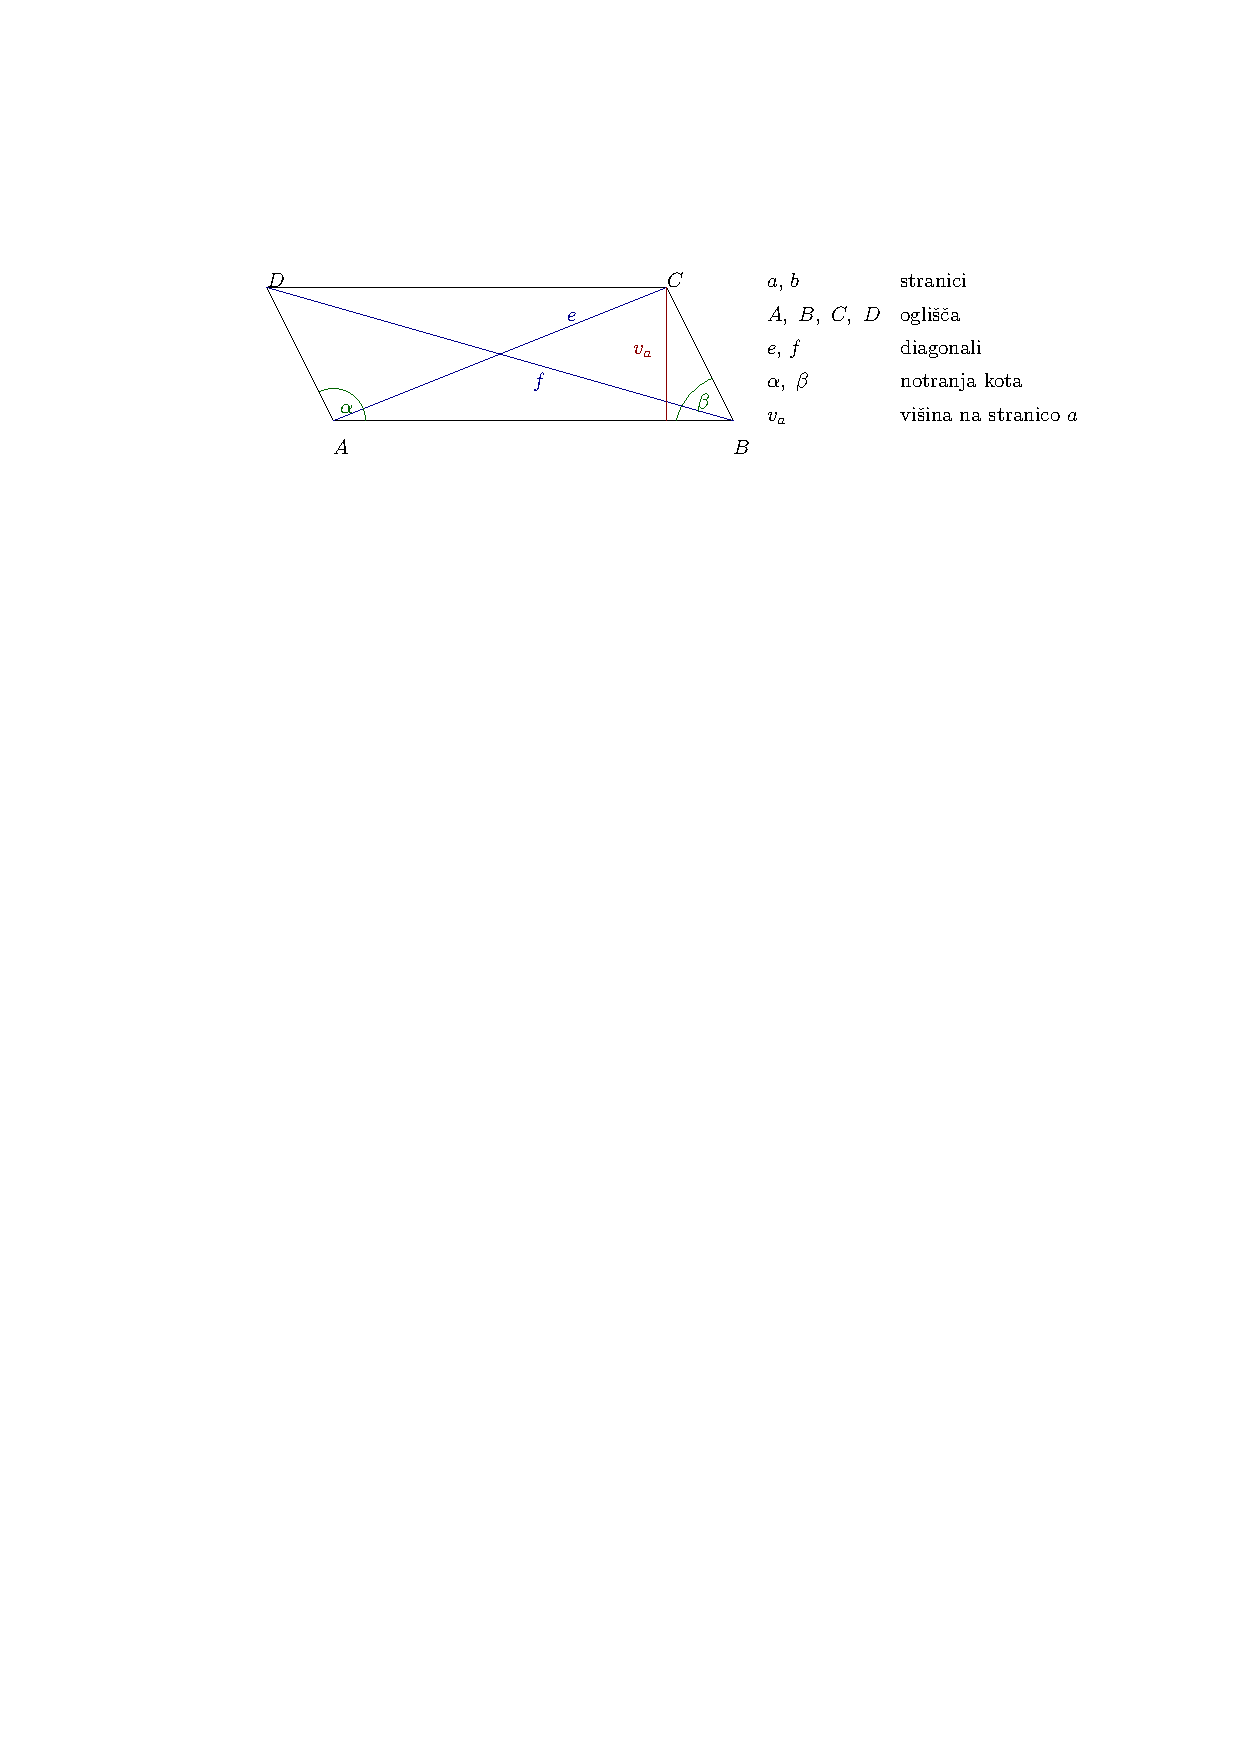
\includegraphics[width=1\textwidth]{paralelogram.pdf}
    \centering
\end{figure}

\begin{enumerate}[i]
    \item Dva para vzporednih stranic
    \item Diagonali se razpolavljata
    \item Poljuna sosednja kota sta suplementarna
    \item Poljubna nasprotna kota sta enako veliko
  \end{enumerate}


Pravokotnik = pravokotni paralelogram

Romb = enakostranični paralelogram (diagonali se razpolavljata pod pravim kotom)

Kvadrat = enakostranični pravokotnik

Trapez = štirikotnik, ki ima par vzporednih stranic ($\alpha$ in $\delta$ suplementarna) (enakokraki trapez)

Srednjica trapeza (povezuje razpolovišči krakov in je vzporedna osnovnicama) ima dolžino $s=\frac{a+c}{2}$

Deltoid = štirikotnik, ki ima dva para sosednjih enako dolgih stranic (diagonali sta pravokotni, ena se z drugo razpolavlja \& dva notranja kota sta skladna).

\begin{figure}[H]
    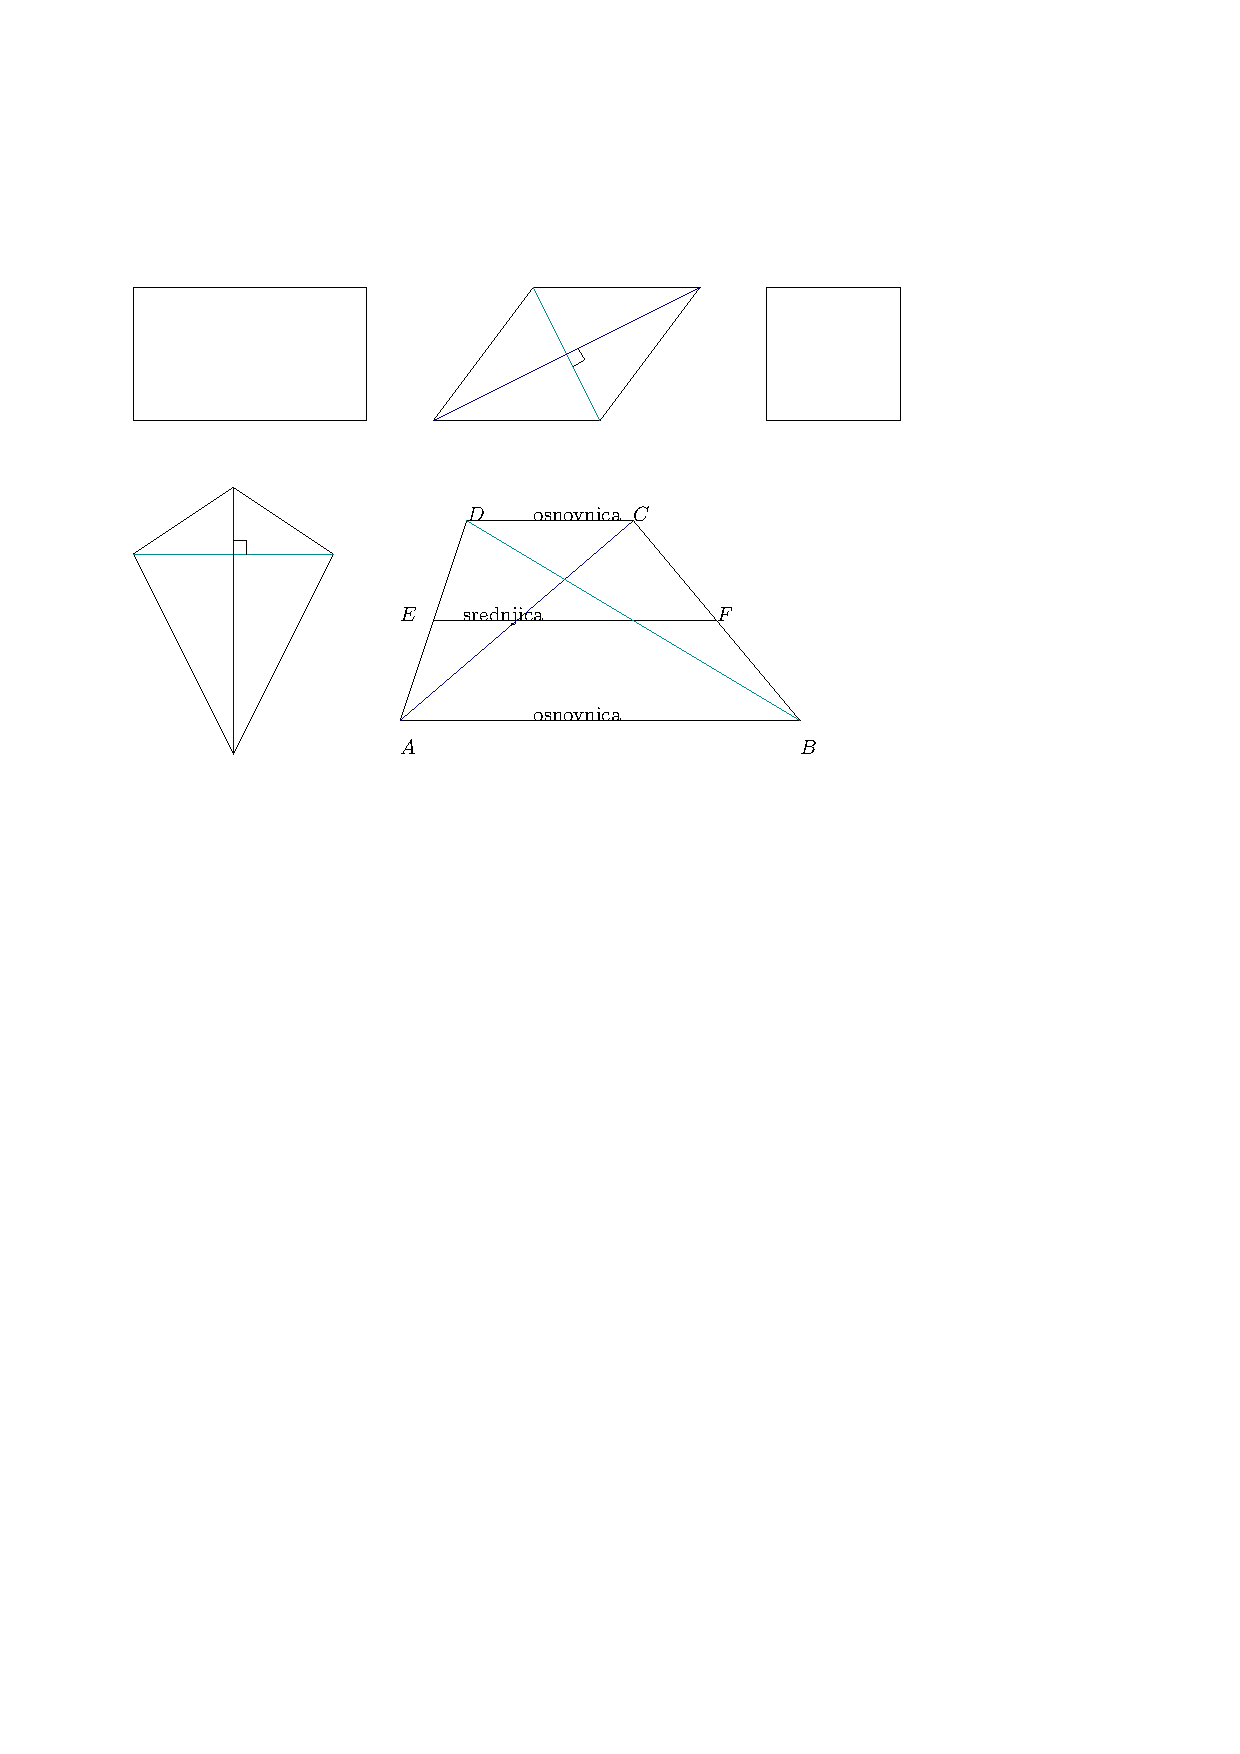
\includegraphics[width=1\textwidth]{liki.pdf}
    \centering
\end{figure}

\begin{zgled}
    Nariši paralelogram $ABCD$, za katerega velja $\alpha=120\degree,\ e=2.5cm,\ v_a=2cm$.
\end{zgled}

\begin{zgled}
    Nariši romb $ABCD$, katerega diagonali merita $e=5cm$ in $f=4cm$.
\end{zgled}

\begin{zgled}
    Nariši pravokotnik $ABCD$, za katerega velja $a=4cm$ in $f=6cm$.
\end{zgled}

\begin{zgled}
    Nariši trapez $ABCD$, za katerega velja $a=4.5cm$, $\beta=45\degree$, $e=3.3cm$ in $f=5cm$.
\end{zgled}

\begin{zgled}
    Nariši trapez $ABCD$, za katerega velja $\alpha=60\degree$, $d=3cm$, $c=2cm$ in $f=6cm$.
\end{zgled}

\begin{zgled}
    Nariši deltoid $ABCD$, za katerega velja $e=4cm$, $f=7cm$ in $a=5cm$.
\end{zgled}

\begin{example}
    DN
\end{example}


Tangentni štirikotnik (očrtamo krožnico, $a+c=b+d$ z dokazom)

Tetivni štirikotnik (včrtamo krožnico, $\alpha+\gamma=\beta+\delta=180\degree$ z dokazom)

Pravilni $n$-kotnik - vse stranice in notranji koti enaki. Vsota kotov = $(n-2)180\degree$. 

\begin{figure}[H]
    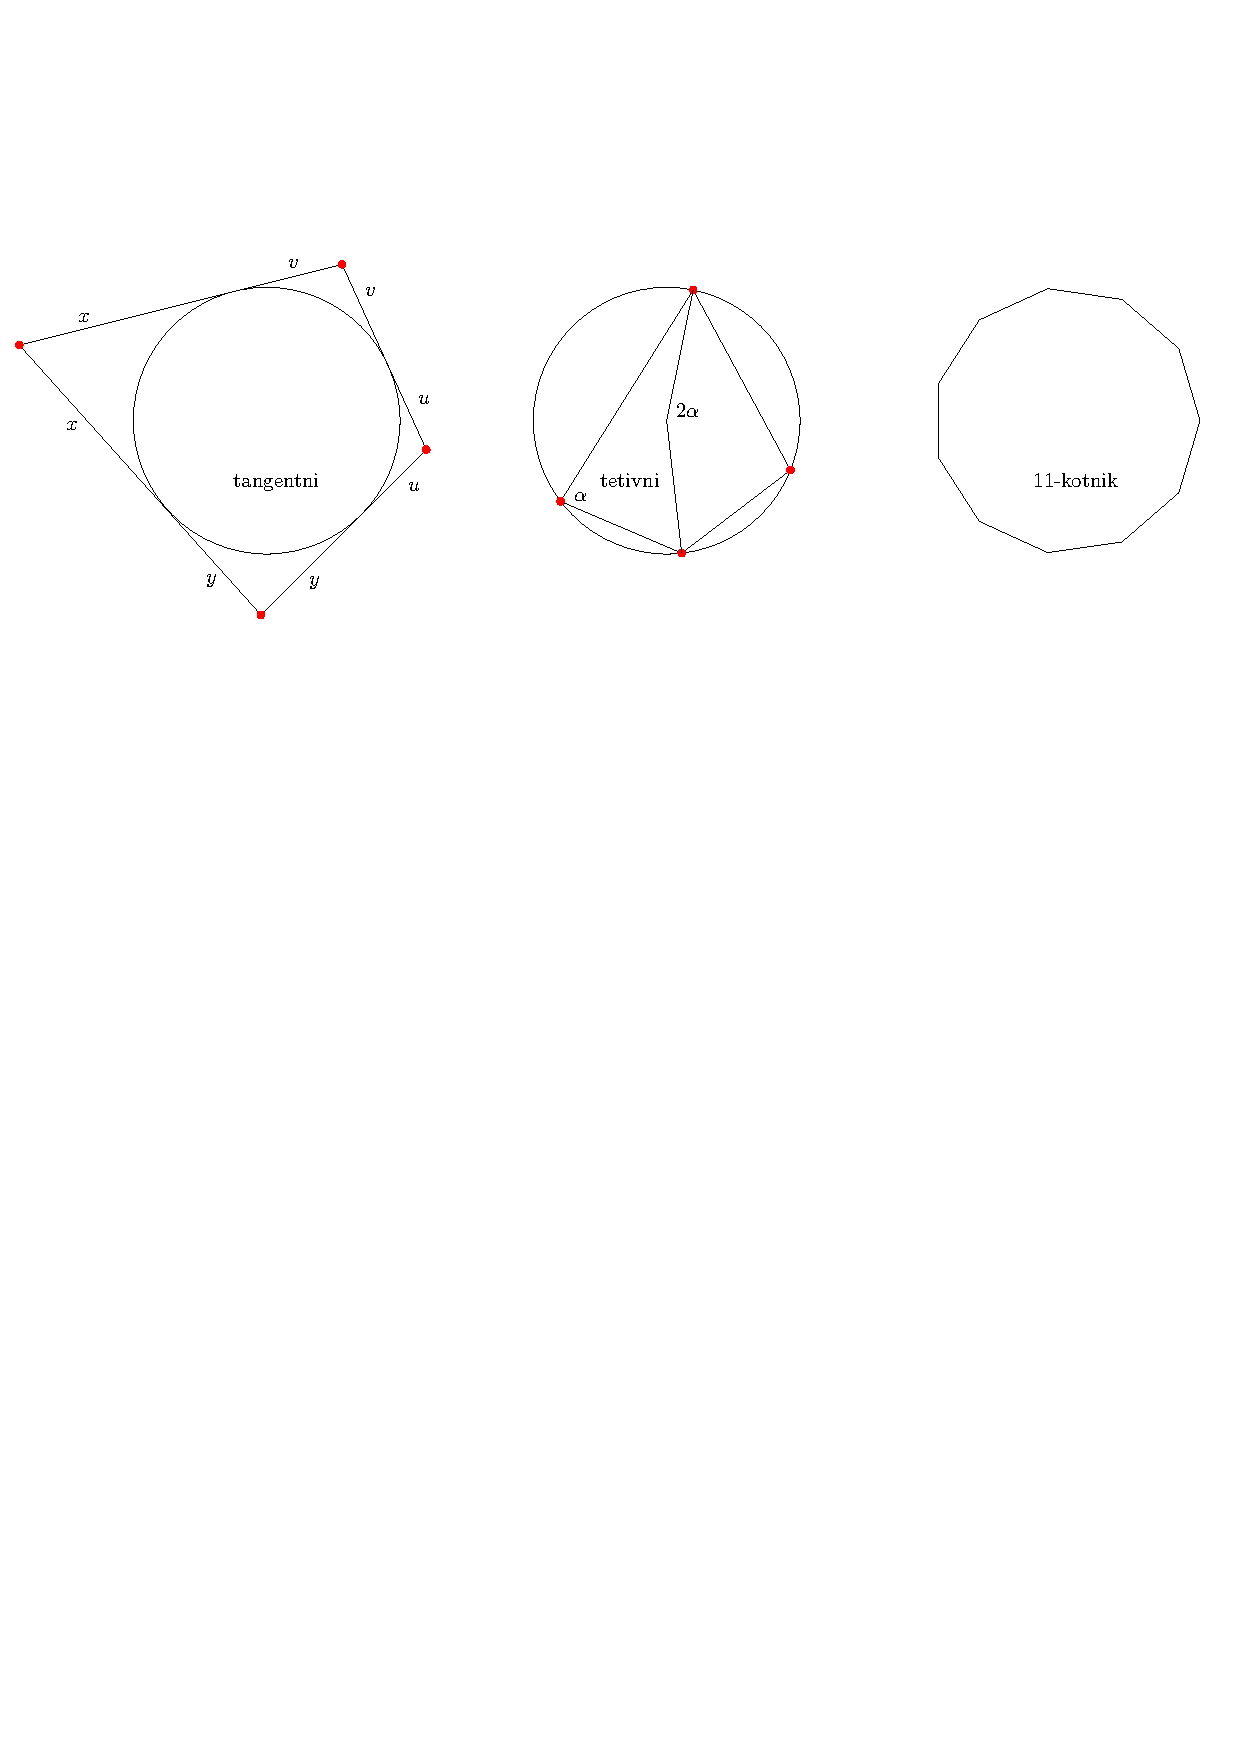
\includegraphics[width=1\textwidth]{liki_2.pdf}
    \centering
\end{figure}

\begin{zgled}
    Glede na sliko določi $|XY|$ in $\angle XYZ$.
    \begin{figure}[H]
    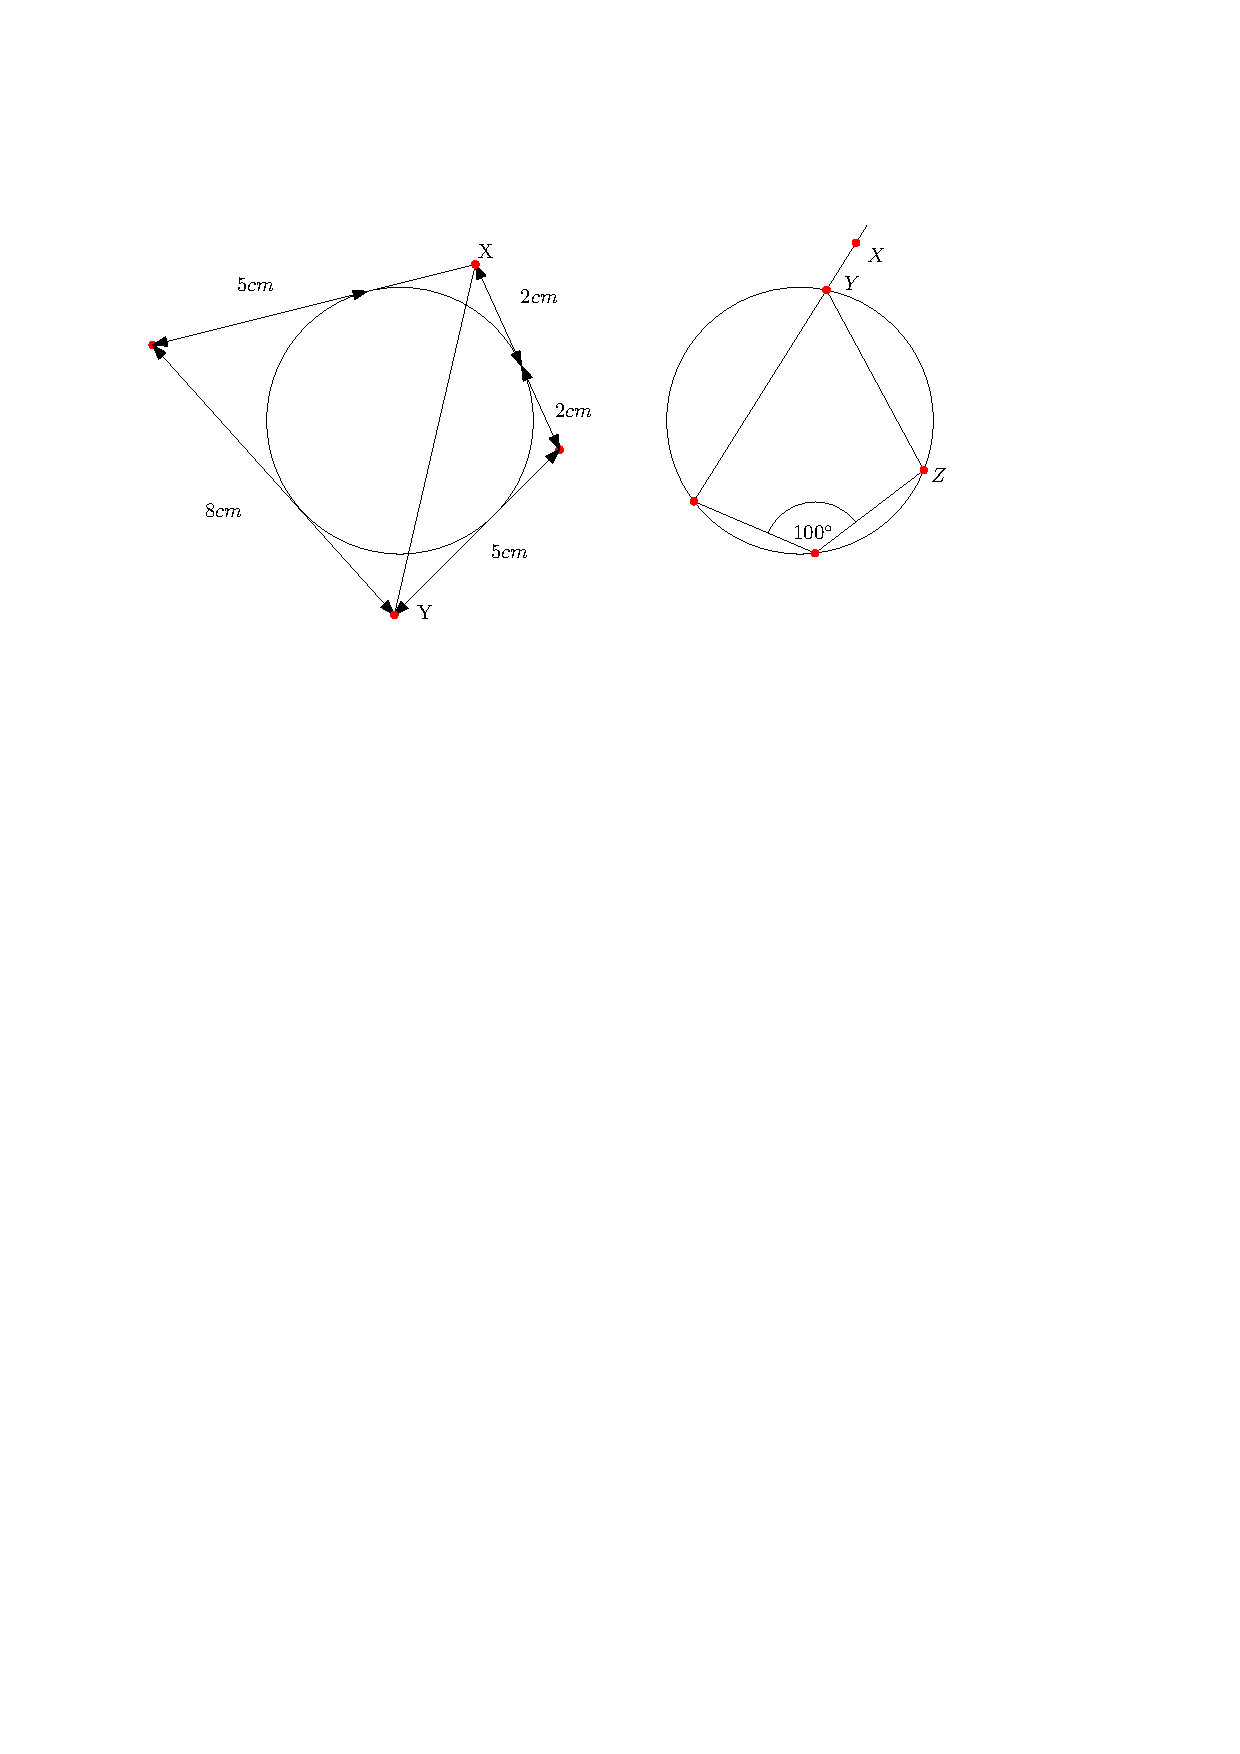
\includegraphics[width=0.8\textwidth]{naloga.pdf}
    \centering
    \end{figure}
\end{zgled}

\begin{zgled}
    Če $n$-kotniku podvojimo število stranic, se njegovor število diagonal pomnoži z $5$. Kateri $n$-kotnik je to.
\end{zgled}

\begin{example}
    DN
\end{example}


\section{Podobnost}


\end{document}